\section{Hely és orientáció feladatok}

%%%%%%%%%%%%%%%%%%%%%%%%%%%%%%%%%%%%%%%%%%%%%%%%%%%%%%%%%%%%%%%%%%%%%%%%%%%%%%%%%%%%%%%%%%%%%%%%%%%%%%%%%%%%
\begin{execise}
	Írjuk fel azt a forgatási mátrixot, amely először az Y tengely körül forgat 30 fokot, majd az X tengely körül forgat 20 fokot!
\end{execise}
\begin{answer}
	Első lépésként írjuk fel a két tengely körüli forgatást jelképező mátrixokat:
	\begin{equation*}
		R_Y=\begin{bmatrix}
			\cos 30^\circ & 0 & \sin 30^\circ \\
			0 & 1 & 0 \\
			-\sin 30^\circ & 0 & \cos 30^\circ \\
		\end{bmatrix}
		\qquad
		R_X=\begin{bmatrix}
		1 & 0 & 0 \\
		0 & \cos 20^\circ & -\sin 20^\circ \\
		0 & \sin 20^\circ & \cos 20^\circ \\
		\end{bmatrix}
	\end{equation*}
	A teljes forgatási mátrix a két mátrix szorzata. Ne feledjük el, hogy a szorzásokat fordított sorrendben kell elvégezni a transzformációkhoz képest!
	\begin{equation*}
	R = R_X R_Y
	\end{equation*}
	
	Magát a forgatási mátrixot MATLAB vagy Octave segítségével könnyen kiszámíthatjuk:
	\begin{lstlisting}
octave:1> Ry=[cosd(30),0,sind(30); 0,1,0; -sind(30),0,cosd(30)]
	Ry =
	
	0.86603   0.00000   0.50000
	0.00000   1.00000   0.00000
	-0.50000   0.00000   0.86603
	
octave:2> Rx=[1,0,0;0,cosd(20),-sind(20);0,sind(20),cosd(20)]
	Rx =
	
	1.00000   0.00000   0.00000
	0.00000   0.93969  -0.34202
	0.00000   0.34202   0.93969
	
octave:3> R=Rx*Ry
	R =
	
	0.86603   0.00000   0.50000
	0.17101   0.93969  -0.29620
	-0.46985   0.34202   0.81380
	\end{lstlisting}
\end{answer}

%%%%%%%%%%%%%%%%%%%%%%%%%%%%%%%%%%%%%%%%%%%%%%%%%%%%%%%%%%%%%%%%%%%%%%%%%%%%%%%%%%%%%%%%%%%%%%%%%%%%%%%%%%%%
\begin{execise}
	Legyen egy három dimenziós forgatási mátrix 
	\begin{equation*}
	\mathbf{R}=\begin{bmatrix}
	0.5 & 0.5 & \frac{\sqrt{2}}{2} \\
	0.5 & 0.5 & -\frac{\sqrt{2}}{2} \\
	-\frac{\sqrt{2}}{2} & \frac{\sqrt{2}}{2} & 0 \\
	\end{bmatrix}
	\end{equation*}
	Határozzuk meg a forgatás tengelyét és szögét!
\end{execise}
\begin{answer}
	Egy forgatási mátrix tengelye ($\mathbf{v}$) a forgatás során nem változik, tehát az a forgatás sajátvektora, valamint a hozzá tartozó sajátérték $\lambda=1$, hiszen $\mathbf{R}\mathbf{v}=\mathbf{v}$, amiből $(\mathbf{R}-\mathbf{I})\mathbf{v}=0$. Tehát keressük az a $\mathbf{v}$ vektort, amelyre:
	\begin{equation*}
	(\mathbf{R}-\mathbf{I})\mathbf{v}=\begin{bmatrix}
	-0.5 & 0.5 & \frac{\sqrt{2}}{2} \\
	0.5 & -0.5 & -\frac{\sqrt{2}}{2} \\
	-\frac{\sqrt{2}}{2} & \frac{\sqrt{2}}{2} & -1 \\
	\end{bmatrix}\mathbf{v}=0
	\end{equation*}
	A középső sor megfelelő skalárszorosát kivonva az első és utolsó sorból (megtehetjük, hiszen az egyenlet homogén), kapjuk, hogy
	\begin{equation*}
	\begin{bmatrix}
	0 & 0 & 0 \\
	1 & -1 & -\sqrt{2} \\
	0 & 0 & -2 \\
	\end{bmatrix}
	\begin{bmatrix}
	v_x \\ v_y \\ v_z \\
	\end{bmatrix}=
	\begin{bmatrix}
	0 \\ 0 \\ 0 \\
	\end{bmatrix}
	\end{equation*}
	Nyilvánvaló, hogy a tengely a $\mathbf{v}=\left[1,1,0\right]^T$ vektorral párhuzamos, origón áthaladó egyenes (behelyettesítéssel láthatjuk). Az egyenlet persze megoldható tetszőleges másik módszerrel (pl. Gauss elimináció, SVD felbontás). A szög megállapításához válasszunk egy erre merőleges vektort, például az $\mathbf{a}=\left[0,0,1\right]$ vektort (hiszen $\mathbf{a}\mathbf{v}=0$)! Könnyű észrevenni, hogy $\mathbf{R}\mathbf{a} \perp \mathbf{a}$, így a forgatás szöge 90 fok.
\end{answer}

%%%%%%%%%%%%%%%%%%%%%%%%%%%%%%%%%%%%%%%%%%%%%%%%%%%%%%%%%%%%%%%%%%%%%%%%%%%%%%%%%%%%%%%%%%%%%%%%%%%%%%%%%%%%
\begin{execise}
	Írjuk fel a $\mathbf{v}=\left[1,2,3\right]$ tengely körüli $\alpha=40^\circ$ forgatáshoz tartozó forgatási kvaterniót! Írjuk fel az ugyanekkora szöggel, de az X tengely körüli forgatást jelképező kvaterniót!
\end{execise}
\begin{answer}
	Emlékezzük vissza, hogy egy tengely körüli forgatást jelképező kvaterniót az alábbi képlettel írhatjuk fel:
	\begin{equation*}
	\mathbf{q} = e^{\frac{\theta}{2}{(u_x\mathbf{i} + u_y\mathbf{j} + u_z\mathbf{k})}} = \cos \frac{\theta}{2} + (u_x\mathbf{i} + u_y\mathbf{j} + u_z\mathbf{k}) \sin \frac{\theta}{2}
	\end{equation*}
	Fontos kiemelni, hogy a forgatást jelképező tengely \textbf{egységvektor} kell legyen! Tehát,
	\begin{equation*}
	\mathbf{u}=\frac{\mathbf{v}}{\|\mathbf{v}\|}=\left[\frac{1}{\sqrt{14}},\frac{2}{\sqrt{14}},\frac{3}{\sqrt{14}}\right]
	\end{equation*}
	Ebből már nagyon egyszerű a forgatási kvaternió felírása:
	\begin{equation*}
	\mathbf{q} = \cos 20^\circ + (\frac{1}{\sqrt{14}}\mathbf{i} + \frac{2}{\sqrt{14}}\mathbf{j} + \frac{3}{\sqrt{14}}\mathbf{k}) \sin 20^\circ
	\end{equation*}

	\begin{center}
		$\Diamond$
	\end{center}

	Hasonlóképpen, a X tengely körüli forgatáshoz felírhatjuk a tengelyt, mint egységvektort:
	\begin{equation*}
	\mathbf{u}=\left[1,0,0\right]
	\end{equation*}
	, amiből a forgatási kvaternió:
	\begin{equation*}
		\mathbf{q} = \cos 20^\circ + \mathbf{i} \sin 20^\circ
	\end{equation*}
\end{answer}

%%%%%%%%%%%%%%%%%%%%%%%%%%%%%%%%%%%%%%%%%%%%%%%%%%%%%%%%%%%%%%%%%%%%%%%%%%%%%%%%%%%%%%%%%%%%%%%%%%%%%%%%%%%%
\begin{execise}
	Forgassuk el a $\mathbf{p}=\left[1,2,1\right]$ vektort a $\mathbf{u}=\left[1,1,1\right]$ tengely körül 30 fokkal! Oldjuk meg a feladatot kvaterniók és a Rodrigues formula segítségével is!
\end{execise}
\begin{answer}
	Első lépésként vegyük fel az egyes változókat:
\begin{lstlisting}
u=[1,1,1];
p=[1,2,1];
a=30;
\end{lstlisting}

Normalizáljuk a tengely vektorát, hiszen látható, hogy $\|\mathbf{u}\|\neq 1$. Ez egy nagyon fontos lépés, hiszen a kvaternió elkészítéséhez egységvektorra van szükségünk:	
\begin{lstlisting}
u=u/norm(u);
\end{lstlisting}	

Ezután már létrehozhatjuk a forgatáshoz szükséges kvaterniót a $\mathbf{q} = \cos \frac{\theta}{2} + (u_x\mathbf{i} + u_y\mathbf{j} + u_z\mathbf{k}) \sin \frac{\theta}{2}$ képlet alapján MATLAB alatt:	
\begin{lstlisting}
q=[cosd(a/2),u(1)*sind(a/2),u(2)*sind(a/2),u(3)*sind(a/2)];
\end{lstlisting}

Természetesen a forgatni kívánt vektort is kvaternióvá kell alakítanunk a $\mathbf{v} = p_x\mathbf{i} + p_y\mathbf{j} + p_z\mathbf{k}$ formában, hogy egy tiszta kvaterniót kapjunk:
\begin{lstlisting}
v=[0,p(1),p(2),p(3)];
\end{lstlisting}

A forgatást végül a $\mathbf{p'} = \mathbf{q} \mathbf{p} \mathbf{q}^{-1}$ képlet alapján tudjuk elvégezni. Ehhez szükség van a forgatási kvaternió inverzére $\mathbf{q}^{-1}=\dfrac{\mathbf{q}^*}{\|\mathbf{q}\|^2}$:
\begin{lstlisting}
qinv=[q(1) -q(2:4)]/norm(q)^2;
\end{lstlisting}

A szorzás során kihasználjuk a $(q_0 + \mathbf{q})(p_0 + \mathbf{p})=q_0 p_0 + q_0 \mathbf{p} + p_0 \mathbf{q} - \mathbf{q}\cdot\mathbf{p} + \mathbf{q} \times \mathbf{p}$ egyenlőséget:
\begin{lstlisting}
res = [q(1)*v(1) - dot(q(2:4),v(2:4)), q(1)*v(2:4) + v(1)*q(2:4) + cross(q(2:4),v(2:4))];
res = [res(1)*qinv(1) - dot(res(2:4),qinv(2:4)), res(1)*qinv(2:4) + qinv(1)*res(2:4) + cross(res(2:4),qinv(2:4))];
\end{lstlisting}

Itt a \code{pvQ} változó fogja tárolni az elforgatott vektort, ahol az elforgatott vektort az imaginárius részek tartalmazzák. A teljes kód alul látható:
\begin{lstlisting}
u=[1,1,1];
p=[1,2,1];
a=30;

u=u/norm(u);

q=[cosd(a/2),u(1)*sind(a/2),u(2)*sind(a/2),u(3)*sind(a/2)];
v=[0,p(1),p(2),p(3)];

qinv=[q(1) -q(2:4)]/norm(q)^2;
res = [q(1)*v(1) - dot(q(2:4),v(2:4)), q(1)*v(2:4) + v(1)*q(2:4) + cross(q(2:4),v(2:4))];
res = [res(1)*qinv(1) - dot(res(2:4),qinv(2:4)), res(1)*qinv(2:4) + qinv(1)*res(2:4) + cross(res(2:4),qinv(2:4))];
\end{lstlisting}

A Rodrigues formula segítségével is könnyen elvégezhetjük a forgatást. Itt is először felveszzük a bemeneti adatokat, majd a tengely vektorát normalizáljuk.
\begin{lstlisting}
u=[1,1,1];
p=[1,2,1];
a=30;

u=u/norm(u);
\end{lstlisting}

Ezután létrehozzuk a keresztszorzat mátrixot az
\begin{equation*}
[\mathbf{u}]_\times=\begin{bmatrix}
0 & -z & y \\
z & 0 & -x \\
-y & x & 0 \\
\end{bmatrix}
\end{equation*}
képlet alapján.
\begin{lstlisting}
K=[0 -u(3) u(2)
u(3) 0 -u(1)
-u(2) u(1) 0];
\end{lstlisting}

Ezután a Rodrigues formulát alkalmazzuk ($\mathbf{R}=\mathbf{I}+\sin\phi[\mathbf{u}]_\times+(1-\cos\phi)[\mathbf{u}]^2_\times$), majd egyszerű mátrixszorzással elvégezzük a forgatást:
\begin{lstlisting}
R=eye(3)+sind(a)*K+(1-cosd(a))*K*K;
pvRodr=R*p';
\end{lstlisting}

A teljes kód itt található:
\begin{lstlisting}
u=[1,1,1];
p=[1,2,1];
a=30;

u=u/norm(u);

K=[0 -u(3) u(2)
u(3) 0 -u(1)
-u(2) u(1) 0];
R=eye(3)+sind(a)*K+(1-cosd(a))*K*K;
pvRodr=R*p';
\end{lstlisting}

\end{answer}

%%%%%%%%%%%%%%%%%%%%%%%%%%%%%%%%%%%%%%%%%%%%%%%%%%%%%%%%%%%%%%%%%%%%%%%%%%%%%%%%%%%%%%%%%%%%%%%%%%%%%%%%%%%%
\begin{execise}
	Egy nyugalomban lévő okostelefon gyorsulásérzékelő szenzora az $\textbf{a}=\left[0.28\frac{m}{s^2},-0.108\frac{m}{s^2},9.936\frac{m}{s^2}\right]$ értéket mutatja egy adott pillanatban, míg a mágneses szenzor a $\textbf{h}=\left[18.75\mu T,10.31\mu T,-44.43\mu T\right]$ értéket. Határozzuk meg a telefon megközelítő orientációját egy olyan koordinátarendszerben, ahol az Y tengely észak irányába mutat, a Z tengely az föld középpontjával ellentétes irányba, és az X tengely ezekre jobbkéz szerint merőleges (a koordinátarendszereket lásd. az ábrán)!
	\begin{center}
		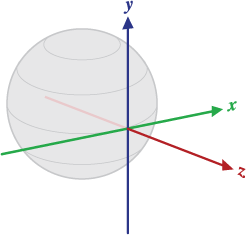
\includegraphics[height=5cm]{fig//axis_globe.png}
		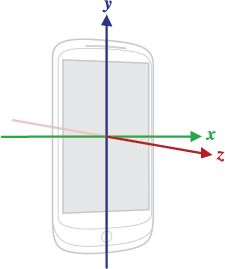
\includegraphics[height=5cm]{fig//axis_device.png}
	\end{center}
\end{execise}
\begin{answer}
	Amint azt tudjuk, a mágneses vektor és a gyorsulás vektor (jelen esetben a nyugalmi helyzet miatt a gravitáció) segítségével 3 szabadságfokú orientációt határozhatunk meg. A két vektor a telefon koordinátarendszerében (az ábrán a jobb oldalon) értelmezett. Vizsgáljuk meg a két vektort!
	\begin{lstlisting}
a=[0.28,-0.108,9.936]
h=[18.75,10.31,-44.43]
	
alength=norm(a)
hlength=norm(h)
	
%	alength =  9.9405
%	hlength =  49.314
	
	\end{lstlisting}
	Láthatjuk, hogy a mágneses térerősség nagyjából $49.314\mu T$ értékű, míg a gyorsulás $9.9405\frac{m}{s^2}$ értékű, amely utóbbi közel esik az elfogadott $9.81\frac{m}{s^2}$ értékhez. Tudjuk, hogy a gravitációs vektor megközelítőleg a föld közepe felé mutat, tehát ,,függőleges''. Ugyanakkor a gyorsulás vektor éppen ellentétes a gravitációs vektorral, hiszen nyugalomban az ellenerő éppen ellentétesen mutat. Tehát az $\mathbf{a}$ vektorunk az \emph{ég felé mutat}, azaz $\mathbf{g}=-\mathbf{a}$!
	
	Mi a helyzet a mágneses vektorral? Ez utóbbi egyrészt nem a valós észak felé mutat (ezt most elhanyagoljuk), másrészt nem is vízszintes. Tekintsük a bezárt szögüket:
	\begin{lstlisting}
a=a/norm(a)
h=h/norm(h)
angle=acosd(dot(a,h))

% angle =  153.14
	\end{lstlisting}
	Itt normalizáltuk a két vektor hosszát, majd egyszerű skaláris szorzattal kiszámítottuk a bezárt szögüket fokban. Mivel az $\mathbf{a}$ vektorunk függőlegesen az ég felé mutat, azt mondhatjuk, hogy a mágneses vektorunk meredeken a föld felé mutat, ez azonban nem meglepetés a 47-dik szélességi fok környékén. A fontos az, hogy a két vektor \emph{nem merőleges} egymásra!
	
	Az orientáció meghatározásához készítsünk először egy merőleges bázisrendszert a vektorainkból! Legyen ez a bázisunk az $\mathbf{x},\mathbf{y},\mathbf{z}$ bázisrendszer. Kérdés, hogy az orientációt melyik vektorra alapozzuk elsősorban? Mivel a függőleges irányt sokkal pontosabban mutatja a gyorsulási vektor, mint az északi irányt a mágneses vektor (hiszen az nem csak északra, hanem lefelé is mutat), használjuk a gyorsulási vektort. Legyen $z=-\mathbf{a}$, tehát a gravitációs vektor iránya. Válasszuk az $\mathbf{x}$ irányt merőlegesnek jobbkéz szabály szerint a gravitációs vektor és mágneses vektor által megadott síkra, azaz $\mathbf{x}=\frac{\mathbf{z}\times\mathbf{h}}{\|\mathbf{z}\times\mathbf{h}\|}$ (itt a vektort egy lépésben normalizáltuk). Az $\mathbf{y}$ irányt pedig természetesen válasszuk merőlegesnek mindkét vektorra, azaz $\mathbf{y}=\mathbf{x}\times\mathbf{z}$ (nincs szükség normalizálásra, hiszen mindkét vektor egység hosszúságú és merőlegesek egymásra)! Ugyanezek a lépések MATLAB-ban:
	\begin{lstlisting}
z=-a
x=cross(z,h)
x=x/norm(x)
y=cross(x,z)
	\end{lstlisting}
	
	Az orientáció meghatározásához már csak a forgatási mátrixot kell felírnunk, amely természetesen a két koordinátarendszer bázisvektorainak a viszonyát írja le. Vegyük észre, hogy a $\mathbf{z}$ vektorunk a gravitáció vektora a \emph{telefon koordinátarendszerében}! Ugyanígy, az $\mathbf{y}$ vektor a mágneses vektor merőleges komponense a gravitációs vektorra a \emph{telefon koordinátarendszerében}. Ebből tehát az orientációs mátrix:
	\begin{equation*}
	R_{\text{earth to phone}}=\begin{bmatrix}
		\mathbf{x}^T & \mathbf{y}^T & -\mathbf{z}^T \\
	\end{bmatrix}
	\end{equation*}
	Az utolsó oszlopot meg kell szoroznunk mínusz eggyel, hiszen a gravitációs vektor a globális koordinátarendszerben pont ellentétesen mutat a Z tengely irányával. A kapott orientációs mátrix az a transzformáció, amely a \emph{globális koordinátarendszer pontjait transzformálja a telefon koordinátarendszerébe}.
	
	\begin{lstlisting}
	a=[0.28,-0.108,9.936]
	h=[18.75,10.31,-44.43]
	
	alength=norm(a)
	hlength=norm(h)
	
	a=a/norm(a)
	h=h/norm(h)
	
	angle=acosd(dot(a,h))
	
	z=-a
	x=cross(z,h)
	x=x/norm(x)
	y=cross(x,z)
	
	R=[x' y' -z']
	\end{lstlisting}
\end{answer}
\bigskip

%%%%%%%%%%%%%%%%%%%%%%%%%%%%%%%%%%%%%%%%%%%%%%%%%%%%%%%%%%%%%%%%%%%%%%%%%%%%%%%%%%%%%%%%%%%%%%%%%%%%%%%%%%%%

\newcommand{\bl}{\mathbf{l}}
\newcommand{\bp}{\mathbf{p}}
\newcommand{\br}{\mathbf{r}}
\begin{execise}
	Tegyük fel, hogy egy klasszikus, kétdimenziós távolságmérésen alapuló helymeghatározási rendszerünk létezik. A rendszerben 5 darab fix helyen található horgonypont (ún. anchor) található, melyektől egy mozgó eszköz valamilyen technológia segítségével megméri a távolságát (minden mérés esetében 5 távolságadat). Határozza meg a felhasználó helyzetét Newton-Gauss iteráció, Kalman-szűrő és RANSAC algoritmus segítségével!
	
	A feladathoz három Octave file tartozik, melyekben a kiindulási adatok találhatók:
	\begin{description}
		\item[anchors.mat] A horgonypontok koordinátáit tartalmazó mátrix
		\item[measurements] A horgonypontoktól való távolságmérések adatai (távolság és a távolságméréshez tartozó szórás), a mérések 100 ms időközönként történtek
		\item[real\_loc.mat] A felhasználó valós helyzetét tartalmazó adathalmaz
	\end{description}

	A feladathoz kiindulási pontként használhatjuk a mellékelt fájlokat, melyek bizonyos részfeladatokban segítenek, illetve egy kiindulási csonkot tartalmaz a \code{main.m} fájlban, melynek kiegészítésével a feladatot könnyebben elvégezhetjük.
\end{execise}
\begin{answer}
	Első lépésként töltsük be az adatokat, majd ábrázoljuk azokat.
\begin{lstlisting}	
clear all;
close all;

% Mérések betöltése
%  d(i,j) - i-dik idöpontban az eszköz távolsága a j-dik anchortól
load measurements;

% A mérőeszközök helyzetének betöltése
% anchors(k,1) - az k-dik anchor X koordinátája
% anchors(k,2) - az k-dik anchor Y koordinátája
load anchors;

% Az eszköz valós helyzete a hiba vizsgálatához
% real_loc(i,1) - az i-dik időpontban az eszköz X koordinátája
% real_loc(i,2) - az i-dik időpontban az eszköz Y koordinátája
load real_loc;
\end{lstlisting}
	Az környezet törlése után a \code{load} paranccsal betöltjük a méréseket, és a horgonypontok koordinátáit. A horgonypontok egy \code{anchors} mátrixban találhatok, soronként egy horgonypont, oszlopokban pedig a koordinátáik találhatók. A mérések egy \code{d} mátrixban találhatók, itt minden sor egy-egy időpillanat, az oszlopok pedig az adott időpontban történt távolságmérések. Az első oszlop az első horgonyponttól történt mérés, és így tovább.

	Rajzoljuk ki az egyes horgonypontokat, majd a felhasználó bejárt útvonalát is. A \code{circle} függvény segítségével pedig rajzoljuk ki az egyes időpillanatokban a horgonypontokhoz tartozó méréseket!
\begin{lstlisting}
for step=1:size(d,1)	% Iteráció az időpillanatokra
	clf;
	
	% Horgonypontok kirajzolása
	main_plot=scatter(anchors(:,1),anchors(:,2),'r');
	axis([-12 22 -12 12]);
	axis equal;
	hold on;
	
	% Valós helyzet ábrázolása
	plot(real_loc(1:step,1),real_loc(1:step,2),'rx-','LineWidth',2);
	
	% Távolságok kirajzolása körökként
	for i=1:size(d,2)
	circle(anchors(i,1),anchors(i,2),d(step,i),'b');
	end;
	
	%
	% Az algoritmusokat ide implementáljuk
	%
	
	pause;
end;
\end{lstlisting}
	Láthatóan egy \code{for} ciklusban implementáltuk a kirajzolást, amely időben engedi futtatni az algoritmust, ha lefuttatjuk, akkor a \code{pause} függvény megállítja a futtatást egy gomb megnyomásáig. Így egy billentyű megnyomásával a következő időpillanatra léphetünk, és áttekinthetjük, miként alakul a felhasználó valós helyzete, és a helyhez tartozó távolságmérések.
	
	\paragraph{Mérési modell}
	Adott időpillanatban a mérések egy távolságvektort alkotnak, azaz $\mathbf{d}=\begin{bmatrix}d_1 & d_2 & d_3 & d_4 & d_5\end{bmatrix}$, ahol 
	\begin{equation*}
		d_k=\sqrt{(x-x_k)^2+(y-y_k)^2}
	\end{equation*}
	Az egyenletben a felhasználó helyzete $\mathbf{l}(x,y)$, a horgonypontok koordinátái pedig $\mathbf{p}_k(x_k,y_k)$. A mérési modell tehát
	\begin{equation*}
	\mathbf{d} = \begin{bmatrix}
	d_1 \\ \vdots \\ d_5
	\end{bmatrix} =
    h(\mathbf{l})  =
	\begin{bmatrix}
		\|\mathbf{p}_1 - \mathbf{l}\| \\
		\vdots \\
		\|\mathbf{p}_5 - \mathbf{l}\| \\
	\end{bmatrix}
	\end{equation*}
	Jól látható, hogy ez egy túldefiniált, nem-lineáris egyenletrendszer, mely zárt alakban nem megoldható.
	
	\paragraph{Newton-Gauss iteráció}
	Kezdjük a megoldást a Newton-Gauss implementációval, amely lehetővé teszi, hogy a nem-lineáris egyenletrendszert iteratív módszerrel megoldjuk. A Newton-Gauss iteráció iterációs lépése a következő:
	\begin{equation*}
		\mathbf{l}_{n+1}=\mathbf{l}_{n}-(J^T J)^{-1} J^T (f(\mathbf{l}_n) - \mathbf{d})
	\end{equation*}
	, ahol $\mathbf{l}_{n}$ a felhasználó helye az $n$-dik iterációban, $f$ a mérési modell, $J$ az $f$ függvény Jacobi-mátrixsza, $\mathbf{d}$ a mérési vektor. A Jacobi-mátrix a parciális deriváltakból álló mátrix, azaz:
	\begin{equation*}
	J=\begin{bmatrix}
		\frac{\partial d_1}{\partial x} & 	\frac{\partial d_1}{\partial y} \\
		\vdots \\
		\frac{\partial d_5}{\partial x} & 	\frac{\partial d_5}{\partial y} \\
	\end{bmatrix}
	\end{equation*}
	, ahol a deriváltak
	\begin{equation*}
	\begin{split}
		\frac{\partial d_k}{\partial x}&=\frac{x-x_k}{\sqrt{(x-x_k)^2+(y-y_k)^2}} \\
		\frac{\partial d_k}{\partial y}&=\frac{y-y_k}{\sqrt{(x-x_k)^2+(y-y_k)^2}} \\
	\end{split}
	\end{equation*}
	
	Ebből a Newton-Gauss algoritmus megvalósítása meglehetősen egyszerű MATLAB-ban. Definiáljuk a fájl legelején (a fő iteráción kívül) a Newton-Gauss iteráció eredményeképpen létrejött helyek eltárolására alkalmas mátrixot:
	\begin{lstlisting}
	nghist=[];
	\end{lstlisting}
	Ezután készítsük el a Newton-Gauss iterációt. A példában 10 iterációt alkalmazunk, valós körülmények között természetesen valamilyen leállási feltételre van szükség. Az $\mathbf{l}_n$ iterációs állapotvektort az \code{ngloc} változó tárolja. Az egyes eredményeket végül az \code{nghist} változóba konkatenáljuk, így a Newton-Gauss algoritmus által visszaadott hisztorikus útvonalat ki tudjuk rajzolni (zöld színt használva).
	\begin{lstlisting}
% Newton-Gauss algoritmus, 10 iterációval
ngloc=[0;0];
for iter=1:10
	J=[];	% Jacobi mártix
	
	% A Jacobi mátrix kitöltés soronként (horgonypontonként)
	for ai=1:size(anchors,1)
		J(ai,1)=(ngloc(1)-anchors(ai,1))/sqrt((ngloc(1)-anchors(ai,1))^2+(ngloc(2)-anchors(ai,2))^2);
		J(ai,2)=(ngloc(2)-anchors(ai,2))/sqrt((ngloc(1)-anchors(ai,1))^2+(ngloc(2)-anchors(ai,2))^2);
		
		eps(ai,1)=sqrt((ngloc(1)-anchors(ai,1))^2+(ngloc(2)-anchors(ai,2))^2)-d(step,ai);
	end
	
	% Newton-Gauss iterációs lépés
	ngloc=ngloc-inv(J'*J)*J'*eps;
end

% Historikus útvonal gyüjtése és kirajzolása
nghist=[nghist; ngloc'];
plot(nghist(:,1),nghist(:,2),'gx-','LineWidth',2);
	\end{lstlisting}
	
	\paragraph{Kalman-szűrő}
	Mivel a mérési modellünk nem lineáris, ezért kiterjesztett Kalman-szűrőt kell alkalmaznunk. Legyen a Markov modellünk a következő:
	\begin{equation*}
	\begin{split}
		\mathbf{l}_{i+1} &= \mathbf{l}_i + \mathbf{v}_i\Delta t + \frac{1}{2}\mathbf{a}_i\Delta t^2 \\
		\mathbf{v}_{i+1} &= \mathbf{v}_i + \mathbf{a}_i \Delta t \\
		\mathbf{d}_i &= h(\mathbf{l}_i) + \mathbf{r}	\\
	\end{split}
	\end{equation*}
	, ahol $\mathbf{l}_i=(l_x^i,l_y^i)$ a felhasználó helye az $i$-dik időpillanatban, $\mathbf{v}_i=(v_x^i,v_y^i)$ és $\mathbf{a}_i=(a_x^i,a_y^i)$ rendre a felhasználó sebessége és gyorsulása az $i$-dik időpillanatban, $\mathbf{d}_i$ a távolságmérések az $i$-dik időpillanatban, $h$ a mérési modell (lásd. Newton-Gauss). Ebből az állapotvektorunk
	\begin{equation}
		\mathbf{x}_i=\begin{bmatrix}
			\mathbf{l}_i \\
			\mathbf{v}_i \\
		\end{bmatrix}
	\end{equation}
	
	Feltételezve, hogy a gyorsulás a zaj komponenshez járul hozzá, a teljes dinamikus modellünk a következő:
	\begin{equation}
		\mathbf{x}_{i+1} = F\mathbf{x}_i + G\mathbf{a}_i
	\end{equation}
	ahol
	\begin{equation}
		F=\begin{bmatrix}
			1 & 0 & \Delta t & 0 \\
			0 & 1 & 0 & \Delta t \\
			0 & 0 & 1 & 0 \\
			0 & 0 & 0 & 1 \\
		\end{bmatrix}
	\end{equation}
	\begin{equation}
		G=\begin{bmatrix}
			\frac{1}{2} \Delta t^2 & 0 \\
			0 & \frac{1}{2} \Delta t^2 \\
			\Delta t & 0 \\
			0 & \Delta t \\
		\end{bmatrix}
	\end{equation}
	Az $\mathbf{r}\sim N(0,R)$ zaj normális eloszlású, és az $R$ kovariancia mátrix diagonális, és ismert (\code{dvar} változóban található értékek). A $a_x,a_y\sim N(0,\sigma_a^2)$ zaj ismert, fix kovariancia mátrixszal rendelkezik. Ebből a teljes zaj eloszlása $G\mathbf{a_i} \sim N(0,G \sigma_a^2 G^T)$ A dinamikus modell szerint tehát az eszköz newtoni mozgást végez, és a gyorsulása ismeretlen. A kiterjesztett Kalman-szűrő szerint $\mathbf{l}$ eloszlása is normális, méghozzá $\mathbf{l}\sim N(\mathbf{m},P)$. 
	
	A kiterjesztett Kalman-szűrő megoldási egyenlete tehát:
	\begin{equation}
	\begin{split}
	m_i^- &= m_{i-1} \\
	P_i^- &= P_{i-1}+Q_{i-1} \\
	\\
	v_i &= d_i-h(m_i^-) \\
	S_i &= H_x(m_i^-) P_i^- H_x^T(m_i^-)+R_i \\
	K_i &= P_i^- H_x^T(m_i^-) S_i^{-1} \\
	m_i &= m_i^- + K_i v_i \\
	P_i &= P_i^- - K_i S_i K_i^T \\
	\end{split}
	\end{equation}
	, ahol $F_x$ az $f$ Jacobi-mátrixsza (lásd. Newton-Gauss). Ezek alapján a Kalman-szűrő könnyedén implementálható MATLAB-ban. Kezdetben definiáljuk az alapvető állapotvektorokat és zaj kovarianciákat a fájl elejére:
	\begin{lstlisting}
% Kalman filter állapotvektor
kfhist=[];
m=[];
P=eye(4);

sd=10;		% a gyorsulás szórása
dt=0.1;		% az időalap
A=[1 0 dt 0;
	0 1 0 dt;
	0 0 1 0;
	0 0 0 1;];
G=[.5*dt*dt 0;
	0 .5*dt*dt;
	dt 0
	0 dt];
Q=G*G'*sd*sd;
	\end{lstlisting}
	Itt a dinamikus modell zajának 1 métert adtunk meg, így az eszköz elmozdulását 1 méter szórásra állítottuk, tehát a prediktált pozíciója az előző hely nagyjából 3 méteres körzetében lesz 99\% valószínűséggel.
	\begin{lstlisting}
% Kalman-szürő  
if isempty(m)
	m=ngloc;	% A kezdeti hely a Newton-Gauss iteráció alapján
end;

% Predikciós lépés
m=A*m;
P=A*P*A'+Q;

H=[];
for ai=1:size(anchors,1)
	H(ai,1)=(m(1)-anchors(ai,1))/sqrt((m(1)-anchors(ai,1))^2+(m(2)-anchors(ai,2))^2);
	H(ai,2)=(m(2)-anchors(ai,2))/sqrt((m(1)-anchors(ai,1))^2+(m(2)-anchors(ai,2))^2);
	H(ai,3)=0;
	H(ai,4)=0;
	
	h(ai,1)=sqrt((m(1)-anchors(ai,1))^2+(m(2)-anchors(ai,2))^2);
end
R=diag(dvar(step,:));

% Frissítési lépés
v=d(step,:)'-h;
S=H*P*H'+R;
K=P*H'*inv(S);
m=m+K*v;
P=P-K*S*K';

% Historikus utvonal gyüjtése és kirajzolása
kfhist=[kfhist; m'];
plot(kfhist(:,1),kfhist(:,2),'bx-','LineWidth',2);
circle(kfhist(end,1),kfhist(end,2),P(1,1),'b');	% A hiba mértékének jelzése
	\end{lstlisting}
	A következő fontos megjegyzéseket tesszük. A Kalman-szűrő kezdeti állapotának a Newton-Gauss iteráció eredményét vesszük (csak az első pozíció esetében). Az $R$ kovariancia mátrixot figyeljük meg, hogy a bemeneti adatok alapján töltjük ki, méghozzá diagonál mátrixra, tehát az egyes távolságmérések között nem feltételezünk korrelációt. Az algoritmus végén külön sorban kirajzoljuk a hely szórását is körként, méghozzá a kovariancia mátrix első eleme segítségével (valóságban ez ellipszis is lehetne, vagy akár a kovariancia mátrixban lehetnek nem diagonális elemek is, ezeket most elhanyagoljuk).
	
	\paragraph{RANSAC}
	A RANSAC algoritmusok az ún. robusztus algoritmusok közé tartoznak, melyek lehetővé teszik a felállított sztochasztikus modellünktől eltérő hibák feltárását, és a modellnek nem megfelelő mérések, ún. outlier-ek kiszűrését. A feladatok során csupán a legegyszerűbb, fix iterációszámmal dolgozó (tehát nem adaptív) RANSAC algoritmust implementáljuk.
	
	A megvalósítás során minden iterációban kiválasztunk két mérést, hiszen két mérés esetén két kört kapunk, amelyeknek kettő, egy, vagy nulla metszéspontja lehet. Első esetben véletlenszerűen választunk a két metszéspont közül, az utolsó esetben a két kör középpontját összekötő egyenesen vesszük fel a metszéspontot. A metszéspont ismeretében a méréseket aszerint osztályozzuk inlier és outlier mérésekre, hogy melyik található a pont $\varepsilon=2$ méteres körzetében. Ennek megfelelően összeállítjuk a mérések indexeiből az inlier index halmazt. Amennyiben ez több elemet tartalmaz, mint az eddigi legtöbb elemet tartalmazó halmaz, a legjobb megoldásként kezeljük. Végül az iterációk lejátszása után a legtöbb inlier-t tartalmazó halmazban található méréseket vastagabb körként ábrázoljuk (valóságban ezeket a méréseket használjuk a további becslések során, pl. a Kalman-szűrőben, vagy a Newton-Gauss iterációban).
	
	A RANSAC megvalósítása MATLAB környezetben ezek alapján nyilvánvaló:
	\begin{lstlisting}
% RANSAC
error_threshold=2;	% Az inlier mérések maximális hibája, méterben
best_inlier_idx=[];	% Az iterációk során eddig megtalált legnagyobb inlier halmaz
for iter=1:30
	% Minimális mintahalmaz kiválasztása (2 pont a körök metszéséhez)
	anchor_idx1=randi(size(anchors,1));
	anchor_idx2=randi(size(anchors,1));
	
	% Figyeljünk arra, hogy ne legyen a két index azonos
	while anchor_idx1 == anchor_idx2
		anchor_idx2=randi(size(anchors,1));
	end
	
	% A két kiválasztott horgonyponthoz tartozó távolsági görbék metszete (2 db, ebböl egy kiválasztása véletlenszerüen)
	test_point=circle_intersect(anchors(anchor_idx1,1),anchors(anchor_idx1,2),d(step,anchor_idx1),anchors(anchor_idx2,1),anchors(anchor_idx2,2),d(step,anchor_idx2));
	test_point=test_point(randi(2),:);
	
	% A próbamegoldáshoz tartozó inlierek összegyüjtése
	inlier_idx=[];
	for ai=1:size(anchors,1)
		distance=sqrt((anchors(ai,1)-test_point(1))^2+(anchors(ai,2)-test_point(2))^2);
		if abs(distance-d(step,ai)) < error_threshold
			inlier_idx=[inlier_idx ai];
		end
	end
	
	% Ha a talált megoldás jobb, akkor mentsük le
	if length(inlier_idx) > length(best_inlier_idx)
		best_inlier_idx = inlier_idx;
	end
end
	
% Az inlier távolságok ábrázolása vastagabb körként
for i=best_inlier_idx
	circle(anchors(i,1),anchors(i,2),d(step,i),'LineWidth',2);
end
	\end{lstlisting}
	
	Figyeljük meg, hogy a körök metszéspontját a \code{circle_intersect} függvénnyel végezzük, amely a két kör középpontját és a két kör sugarát várja az argumentumában. A függvényt a \code{circle_intersect.m} fájlban találjuk, és mellékeltük a gyakorlat anyagához.
\end{answer}


